% !TEX root = manuscript.tex

\chapter{Modélisation et Analyse des Résultats}

\section{Introduction aux approches utilisées}

\begin{flushleft}
Notre approche de modélisation pour la reconnaissance des caractères ourdou a suivi une progression méthodique, partant de modèles relativement simples pour évoluer vers des architectures plus sophistiquées. Cette démarche incrémentale nous a permis de comprendre précisément comment chaque niveau de complexité contribue à l'amélioration des performances.

Trois modèles principaux ont été développés et évalués :



\begin{enumerate}
\item \textbf{Perceptron Multicouche (MLP) :} Ce modèle de base, composé uniquement de couches denses entièrement connectées, nous a servi de référence. Il traite les images comme des vecteurs aplatis, sans tenir compte explicitement des relations spatiales entre pixels.
\item \textbf{CNN simple :} Cette architecture introduit des couches de convolution qui peuvent détecter des motifs locaux dans les images. Elle représente une amélioration substantielle par rapport au MLP en exploitant la structure bidimensionnelle des données.

\item \textbf{CNN profond avec BatchNormalization :}  Le modèle le plus avancé incorpore une architecture plus profonde, des mécanismes de régularisation supplémentaires et des techniques d'optimisation modernes pour maximiser les performances. 
\end{enumerate}

Cette progression nous a permis non seulement d'améliorer significativement les résultats, mais aussi d'approfondir notre compréhension des facteurs qui influencent l'efficacité des modèles de deep learning dans les tâches de reconnaissance visuelle.
\end{flushleft}

\section{Modèle 1 : Perceptron Multicouche (MLP)}

\subsection{Architecture}

\begin{flushleft}
Le Perceptron Multicouche constitue notre approche initiale, offrant une base de comparaison pour les modèles plus sophistiqués. L'architecture implémentée (voir Annexe~\ref{sec:annexe2}) se compose de :

\begin{itemize}
\item Une couche d'entrée avec 512 neurones, qui reçoit les 784 pixels aplatis de chaque image
\item Une couche cachée avec 256 neurones
\item Une couche de sortie avec 40 neurones (un pour chaque classe de caractère ourdou)
\item Des fonctions d'activation ReLU pour les couches intermédiaires et softmax pour la couche de sortie
\item Des couches de Dropout avec un taux de 0.2 pour réduire le surapprentissage
\end{itemize}

Le modèle totalise environ 543 000 paramètres entraînables, ce qui représente une complexité modérée mais suffisante pour tenter d'apprendre les motifs distinctifs des caractères ourdou.
\end{flushleft}

\subsection{Entraînement}

\begin{flushleft}
Le MLP a été entraîné avec les paramètres suivants :

\begin{itemize}
\item \textbf{Optimiseur :} Adam avec un taux d'apprentissage de 0.0005
\item \textbf{Fonction de perte :}Entropie croisée catégorielle (categorical\_crossentropy)
\item \textbf{Métrique :} Précision (accuracy)
\item \textbf{Batch size :} 32
\item \textbf{Époques :} 0 maximum, avec arrêt anticipé (early stopping)
\item \textbf{Validation :} 20\% des données d'entraînement

Des callbacks ont été implémentés pour améliorer l'entraînement :

\item \textbf{EarlyStopping} pour arrêter l'entraînement lorsque la perte sur l'ensemble de validation cesse de diminuer
\item \textbf{ModelCheckpoint} pour sauvegarder la meilleure version du modèle
\end{itemize}


L'entraînement s'est stabilisé après environ 7-10 époques, suggérant une convergence relativement rapide mais aussi une capacité limitée du modèle à continuer à apprendre des caractéristiques plus complexes.
\end{flushleft}

\subsection{Résultats(54.6\%)}

\begin{flushleft}
Le MLP a atteint une précision sur l'ensemble de validation de :

\begin{itemize}
\item \textbf{Précision finale :} 54.6\%
\item \textbf{Perte (loss) :} 1.55
\end{itemize}
\bigskip
Cette performance, bien que significativement supérieure à une classification aléatoire (qui donnerait environ 2.5\% pour 40 classes), reste insuffisante pour une application pratique de reconnaissance de caractères. Le modèle montre une capacité limitée à différencier correctement les 40 classes de caractères ourdou.
\bigskip
Un aspect notable de ces résultats est que la meilleure performance a été atteinte dès la première époque d'entraînement, après quoi la qualité des prédictions a stagné ou diminué, suggérant que le modèle a rapidement atteint les limites de sa capacité à modéliser la complexité des données d'image sans tenir compte des relations spatiales entre pixels.
\end{flushleft}

\subsection{Analyse des limites}
\begin{flushleft}
L'analyse des résultats révèle plusieurs limitations inhérentes à l'architecture MLP pour cette tâche :

\begin{enumerate}
\item \textbf{Perte de l'information spatiale :} En aplatissant les images en vecteurs unidimensionnels, le MLP perd la relation spatiale entre pixels adjacents, qui est cruciale pour reconnaître les motifs visuels complexes des caractères ourdou.
\item \textbf{Sensibilité à la position : }Le MLP ne possède pas d'invariance par translation, ce qui signifie qu'un même caractère légèrement déplacé dans l'image peut être perçu comme totalement différent par le modèle. 
\item \textbf{Surapprentissage rapide :}Malgré l'utilisation de Dropout, le modèle montre des signes de surapprentissage, avec un écart croissant entre les performances sur les ensembles d'entraînement et de validation après quelques époques.
\item \textbf{Confusion entre caractères similaires :}L'analyse de la matrice de confusion révèle que le MLP confond fréquemment des caractères visuellement proches, ne parvenant pas à capturer les détails distinctifs subtils.
\item \textbf{}
\end{enumerate}

Ces limitations mettent en évidence la nécessité d'architectures plus adaptées aux données d'image, capables de préserver et d'exploiter les relations spatiales entre pixels.
\end{flushleft}

\section{Modèle 2 : CNN simple}

\subsection{Architecture}

\begin{flushleft}
Pour remédier aux limitations du MLP, nous avons implémenté un réseau de neurones convolutifs (CNN) simple, spécifiquement conçu pour traiter des données d'image. L'architecture (voir Annexe~\ref{sec:annexe3}) introduit plusieurs éléments clés des CNN :

\begin{itemize}
\item Des couches de convolution qui appliquent des filtres pour détecter des motifs locaux dans l'image
\item Des opérations de pooling qui réduisent la dimension spatiale et introduisent une invariance partielle aux translations
\item Une progression du nombre de filtres (32 à 64) qui permet de capturer des motifs de plus en plus complexes
\item Une couche d'aplatissement qui transforme les représentations convolutionnelles en vecteur pour les couches denses finales
\end{itemize}
\bigskip
Le modèle totalise environ 200 000 paramètres, soit moins que le MLP malgré sa capacité accrue à traiter les images, illustrant l'efficacité des opérations de convolution pour l'analyse d'images.
\end{flushleft}

\subsection{Entraînement}
\begin{flushleft}
Le CNN simple a été entraîné avec des paramètres similaires à ceux du MLP :

\begin{itemize}
\item \textbf{Optimiseur :}Adam avec un taux d'apprentissage de 0.001
\item \textbf{Fonction de perte : }Entropie croisée catégorielle
\item \textbf{Batch size :} 64 (augmenté pour exploiter plus efficacement le parallélisme du GPU)
\item \textbf{Époques :}30 maximum, avec early stopping
\end{itemize}
\bigskip

Une différence notable est l'ajout du \textbf{callback ReduceLROnPlateau}, qui réduit automatiquement le taux d'apprentissage lorsque la performance stagne, permettant un réglage plus fin des poids du modèle dans les dernières phases d'entraînement.

\bigskip

L'entraînement du CNN a montré une progression plus stable et continue par rapport au MLP, avec une amélioration constante des performances jusqu'à environ 10-12 époques avant d'atteindre un plateau.
\end{flushleft}

\subsection{Résultats(88\%)}

\begin{flushleft}
Le CNN simple a réalisé une amélioration spectaculaire par rapport au MLP :

\begin{itemize}
\item \textbf{Précision finale :}88.4\%
\item \textbf{Perte (loss) : }0.42
\end{itemize}

\bigskip
Cette amélioration de près de 30 points de pourcentage démontre clairement la supériorité des architectures convolutives pour les tâches de reconnaissance d'images. Le modèle parvient à distinguer correctement la majorité des caractères ourdou, bien que certaines confusions persistent.
\end{flushleft}

\subsection{Analyse des améliorations par rapport au MLP}

\begin{flushleft}
Plusieurs facteurs expliquent cette amélioration significative :

\begin{enumerate}
\item \textbf{Préservation de l'information spatiale : }Les couches de convolution traitent l'image en conservant sa structure bidimensionnelle, permettant au modèle de détecter des motifs locaux et leurs relations spatiales.
\item \textbf{Hiérarchie de caractéristiques :}L'architecture en couches du CNN permet de construire une représentation hiérarchique des caractéristiques, des motifs simples (traits, courbes) aux structures plus complexes qui définissent les caractères.
\item \textbf{Invariance par translation :}Les opérations de pooling rendent le modèle partiellement insensible aux variations de position des caractéristiques, améliorant la robustesse face aux variations mineures dans les images.
\item \textbf{Paramétrage plus efficace :}Bien que moins complexe en termes de nombre total de paramètres, le CNN utilise ces paramètres de manière plus efficace en exploitant la localité des informations visuelles.
\end{enumerate}
\bigskip
Néanmoins, l'analyse de la matrice de confusion (voir Annexe~\ref{sec:annexe6}) révèle que certaines classes restent difficiles à différencier, suggérant qu'une architecture plus sophistiquée pourrait être nécessaire pour capturer les nuances les plus subtiles entre caractères similaires.
\end{flushleft}

\section{Modèle 3 : CNN profond avec BatchNormalization}

\subsection{Architecture détaillée}
\begin{flushleft}
Pour maximiser les performances, nous avons conçu une architecture CNN profonde incorporant plusieurs techniques avancées de deep learning :
\end{flushleft}

\begin{figure}[H]
\centering
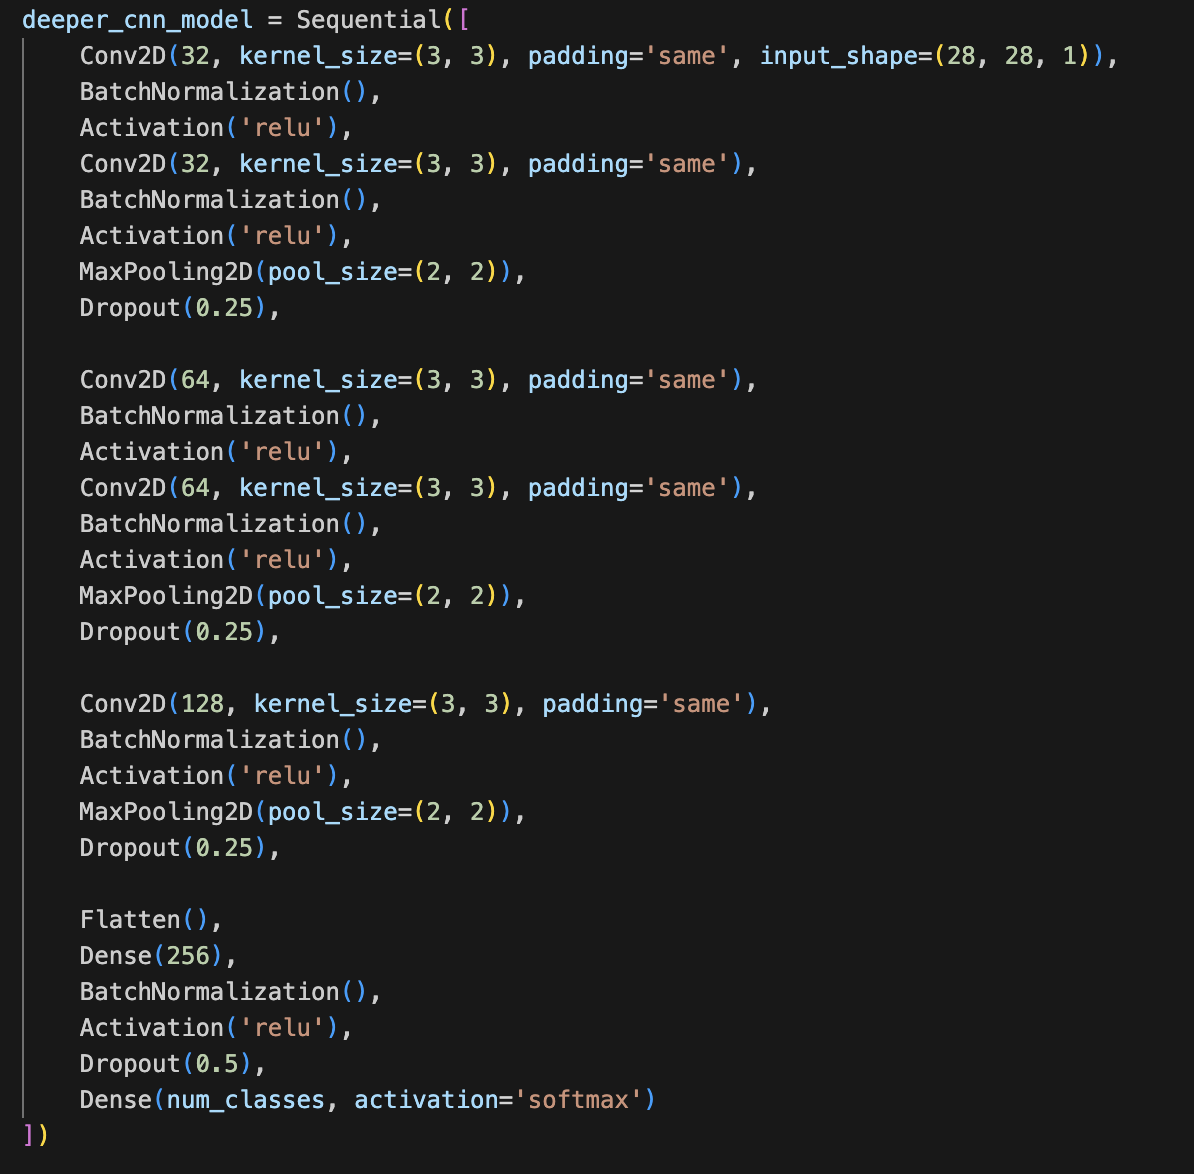
\includegraphics[width=0.7\textwidth]{figures/modeleprofonde.png}
\caption{Architectude du CNN pronfonde}
\label{fig:urdu_CNN}
\end{figure}

\begin{flushleft}
Cette architecture présente plusieurs améliorations significatives :

\begin{enumerate}
\item \textbf{Profondeur accrue :Trois blocs de convolution au lieu de deux, avec une augmentation progressive du nombre de filtres (32->64->128)}
\item \textbf{Convolutions multiples par niveau : }Deux couches de convolution consécutives dans les premiers blocs, permettant d'apprendre des motifs plus complexes
\item \textbf{BatchNormalization :}Après chaque couche de convolution et dense, normalisant les activations pour stabiliser et accélérer l'apprentissage
\item \textbf{Padding 'same' :}Préservant les dimensions spatiales après convolution, permettant d'extraire plus d'informations des bords de l'image
\item \textbf{Dropout stratifié :}Taux de dropout différenciés (0.25 pour les couches convolutives, 0.5 pour la couche dense finale)
\end{enumerate}
\bigskip
Cette architecture totalise environ 446 600 paramètres, représentant un investissement significatif en capacité d'apprentissage, justifié par la complexité de la tâche.
\end{flushleft}

\subsection{Mécanismes de régularisation}

\begin{flushleft}
Le CNN profond intègre plusieurs techniques de régularisation pour éviter le sur-apprentissage malgré sa complexité accrue :

\begin{enumerate}
\item \textbf{BatchNormalization : }Cette technique normalise les activations à chaque couche, ce qui présente plusieurs avantages :
\begin{itemize}
\item Réduction du problème de "covariate shift" interne (changement de distribution des activations)
\item Stabilisation du processus d'apprentissage
\item Accélération de la convergence
\item Effet régularisateur intrinsèque
\end{itemize}
\item \textbf{Dropout adaptatif :} L'utilisation de taux différents selon la profondeur de la couche permet un compromis optimal entre capacité d'apprentissage et généralisation :
\begin{itemize}
\item 25\% dans les couches convolutives pour préserver une partie significative de l'information spatiale
\item 50\% dans la couche dense pour une régularisation plus forte avant la classification finale
\end{itemize}
\item \textbf{Décroissance du taux d'apprentissage : }Le callback \textbf{ReduceLROnPlateau} réduit le taux d'apprentissage lorsque la performance stagne, permettant d'affiner progressivement les poids et d'éviter les oscillations autour du minimum.
\end{enumerate}

\bigskip

Ces mécanismes, combinés à l'early stopping, ont permis de maintenir un bon équilibre entre capacité d'apprentissage et généralisation, comme le montrent les courbes d'apprentissage équilibrées entre entraînement et validation.
\end{flushleft}

\subsection{Résultats (98.5\%)}

\begin{flushleft}
Le CNN profond a atteint des performances exceptionnelles :

\begin{itemize}
\item \textbf{Précision finale sur la validation : }98.5\%
\item \textbf{Perte (loss) : }0.06
\end{itemize}

\bigskip

Cette précision approche les performances humaines pour une tâche de reconnaissance de caractères et représente une amélioration considérable par rapport aux modèles précédents. L'analyse des erreurs résiduelles montre qu'elles concernent principalement des caractères très similaires visuellement, où même un observateur humain pourrait hésiter.
\end{flushleft}

\subsection{Comparaison des performances}

\begin{flushleft}
L'évolution des performances à travers les trois modèles montre une progression remarquable :

\begin{itemize}
\item MLP : 54.6\% de précision
\item CNN simple : 88.4\% de précision
\item CNN profond : 98.5\% de précision
\end{itemize}

\bigskip

Cette amélioration de près de 44 points de pourcentage entre le modèle initial et final illustre l'importance cruciale du choix architectural pour les tâches de reconnaissance visuelle. Elle souligne également comment chaque niveau de sophistication supplémentaire apporte des gains significatifs, en particulier lorsqu'il s'agit de distinguer des caractères présentant des similitudes subtiles.

Cette progression est particulièrement instructive car elle démontre comment l'adaptation de l'architecture du modèle à la nature spécifique des données (dans ce cas, des images) peut conduire à des améliorations spectaculaires des performances, même sans augmentation significative du nombre total de paramètres.


\end{flushleft}

\section{Analyse comparative des trois approches}
\subsection{Tableau comparatif des performances}

\begin{flushleft}
Le tableau suivant synthétise les performances et caractéristiques clés des trois modèles développés :
\end{flushleft}

\begin{table}[H]
\caption{Tableau comparatif des performances}
\label{tab:comparaison}
\resizebox{\textwidth}{!}{%
\begin{tabular}{|c|c|c|c|c|}
\hline
\textbf{Modèle}	&  \textbf{Précision (Validation)} & \textbf{Nombre de paramètres} & \textbf{Temps d'entraînement} & \textbf{Époques jusqu'à convergence} \\ \hline
MLP simple & 58.7\% & 537 000 & 4 minutes & 1 \\
\hline
CNN simple &  88.4\% & 200 000 & 6 minutes & 11 \\
\hline
CNN profond &  98.5\% & 446 600 & 15 minutes & 30 \\
\hline
\end{tabular}%
}
\end{table}

\bigskip

\begin{flushleft}
Ce tableau met en évidence plusieurs tendances intéressantes :

\begin{itemize}
\item Le CNN simple réalise une meilleure performance que le MLP avec moins de paramètres, démontrant l'efficacité des opérations de convolution
\item L'augmentation du temps d'entraînement et du nombre d'époques pour les modèles plus complexes reflète leur capacité à continuer à apprendre des caractéristiques subtiles
\item Le CNN profond nécessite plus de ressources, mais cette investissement se traduit par un gain substantiel en précision
\end{itemize}
\end{flushleft}

\subsection{Analyse des courbes d'apprentissage}


L'analyse des courbes d'apprentissage (voir Annexe~\ref{sec:annexe7}) révèle des différences significatives dans le comportement des trois modèles:


\begin{enumerate}
\item \textbf{MLP:}
\begin{itemize}
\item Meilleure performance atteinte dès la première époque
\item Dégradation constante de la précision de validation après ce pic initial
\item Écart croissant entre précision d'entraînement et validation, avec une augmentation continue de la perte
\item Signes évidents d'instabilité, avec une perte qui augmente dramatiquement à mesure que l'entraînement progresse
\end{itemize}

\item \textbf{CNN simple:}
\begin{itemize}
\item Progression rapide dans les premières époques, suivie d'une amélioration plus graduelle
\item Convergence après environ 10-11 époques
\item Écart modéré mais constant entre les performances d'entraînement et de validation
\item Courbe de perte qui se stabilise, indiquant un processus d'apprentissage plus équilibré
\end{itemize}

\item \textbf{CNN profond:}
\begin{itemize}
\item Progression spectaculaire dès les premières époques, atteignant près de 90\% de précision très rapidement
\item Amélioration continue mais plus lente jusqu'à atteindre des performances optimales
\item Écart remarquablement faible entre précision d'entraînement et validation, surtout dans les phases avancées
\item Courbe de perte qui se stabilise rapidement à des valeurs très basses
\item Faible écart entre entraînement et validation, indiquant une bonne généralisation malgré la complexité accrue
\end{itemize}
\end{enumerate}

\bigskip

Ces graphiques illustrent parfaitement les différences fondamentales entre les trois architectures:


\begin{itemize}
\item Le MLP montre des signes clairs d'inadaptation à la tâche, incapable de maintenir ses performances au-delà de la première époque

\item Le CNN simple présente un bon compromis entre rapidité d'apprentissage et performance, mais atteint un plateau

\item Le CNN profond combine une convergence rapide avec une capacité à continuer à s'améliorer sur de nombreuses époques, tout en maintenant une excellente généralisation grâce à ses mécanismes de régularisation avancés (BatchNormalization, Dropout stratifié)
\end{itemize}

\bigskip

Cette progression visuelle des courbes d'apprentissage confirme l'importance d'adapter l'architecture du modèle à la nature spécifique des données d'image pour des tâches de reconnaissance visuelle complexes.


\subsection{Visualisation des matrices de confusion}

\begin{flushleft}
Les matrices de confusion (voir Annexe~\ref{sec:annexe7}) offrent un aperçu détaillé des forces et faiblesses spécifiques de chaque modèle 

\begin{enumerate}
\item \textbf{MLP:}
\begin{itemize}
\item La diagonale principale est visible mais nettement moins prononcée que pour les autres modèles
\item De nombreuses confusions apparaissent entre classes non liées, avec des points de confusion dispersés à travers toute la matrice
\item Certaines colonnes montrent des concentrations de prédictions incorrectes, indiquant une tendance du modèle à favoriser certaines classes
\item Plusieurs zones claires en dehors de la diagonale révèlent des confusions systématiques entre certains groupes de caractères
\end{itemize}
\item \textbf{CNN simple :}
\begin{itemize}
\item Diagonale principale plus marquée, avec des bleus plus intenses
\item Les confusions sont significativement réduites et plus localisées, généralement entre classes adjacentes ou visuellement similaires
\item Quelques zones persistantes de confusion restent visibles, particulièrement pour certaines classes dans la moitié inférieure de la matrice
\end{itemize}
\item \textbf{CNN profond :}
\begin{itemize}
\item Diagonale principale fortement dominante avec des bleus très intenses
\item Les confusions sont minimales et extrêmement localisées
\item La structure est remarquablement claire, avec presque tous les éléments hors diagonale proches de zéro
\item Les quelques confusions restantes semblent concerner des paires spécifiques de caractères qui partagent probablement des traits visuels très similaires
\end{itemize}
\end{enumerate}

\bigskip 

Cette progression visuelle depuis une matrice relativement diffuse (MLP) vers une matrice clairement dominée par sa diagonale (CNN profond) illustre de façon frappante l'amélioration de la capacité discriminative à chaque niveau architectural. Elle montre comment le CNN profond a réussi à résoudre pratiquement toutes les ambiguïtés entre caractères qui posaient problème aux modèles plus simples.

L'analyse de ces matrices confirme que l'architecture CNN profonde n'apporte pas seulement une amélioration quantitative (en termes de précision globale), mais aussi qualitative, en réduisant drastiquement les confusions entre classes et en améliorant la fiabilité des prédictions à travers l'ensemble des 40 classes de caractères ourdou.
\end{flushleft}

\subsection{Discussion sur les facteurs d'amélioration}

\begin{flushleft}
L'amélioration spectaculaire observée entre les trois modèles peut être attribuée à plusieurs facteurs clés :

\begin{enumerate}
\item \textbf{Préservation de l'information spatiale :} Le passage du MLP au CNN permet de conserver et d'exploiter la structure bidimensionnelle des images, aspect fondamental pour la reconnaissance de caractères.
\item \textbf{Hiérarchie de représentation : }Les architectures CNN permettent d'apprendre des représentations hiérarchiques, des motifs simples aux structures complexes, particulièrement adaptées à la nature des caractères ourdou.
\item \textbf{Profondeur architecturale :}L'augmentation contrôlée de la profondeur du réseau permet d'apprendre des représentations plus abstraites et discriminantes, essentielles pour distinguer des caractères visuellement proches.
\item \textbf{Mécanismes de régularisation avancés :}L'intégration de techniques comme BatchNormalization stabilise l'apprentissage et améliore la généralisation, permettant d'exploiter pleinement la capacité du modèle sans surapprentissage.
\item \textbf{Optimisation adaptative :}L'utilisation de techniques comme la réduction du taux d'apprentissage sur plateau permet d'affiner progressivement les poids du modèle, améliorant la convergence vers des minima plus optimaux.
\end{enumerate}

\bigskip

La combinaison de ces facteurs a permis d'atteindre des performances exceptionnelles dans cette tâche de reconnaissance de caractères ourdou, démontrant l'importance d'une approche progressive et réfléchie dans la conception des architectures de deep learning.
\end{flushleft}

\section{Soumission sur Kaggle et résultats finaux}
\subsection{Soumission sur Kaggle}
\begin{flushleft}
Après avoir sélectionné notre meilleur modèle (CNN profond avec BatchNormalization), nous avons procédé à la génération des prédictions sur l'ensemble de test fourni par la compétition.

\bigskip

Notre soumission a obtenu un score remarquable de 99.1\% sur l'ensemble de test de la compétition, confirmant l'excellente capacité de généralisation de notre modèle sur des données non vues pendant l'entraînement.

\bigskip

Ce résultat place notre solution parmi les plus performantes pour cette tâche de reconnaissance de caractères ourdou, validant l'efficacité de l'approche progressive que nous avons adoptée, depuis le MLP simple jusqu'au CNN profond avec techniques de régularisation avancées.

\bigskip 

Voici un aperçu du fichier de soumission:
\end{flushleft}

\begin{figure}[h]
\centering
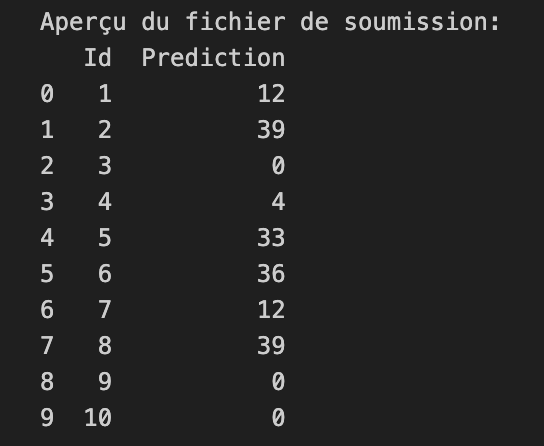
\includegraphics[width=0.7\textwidth]{figures/Soumission.png}
\caption{Apercu du fichier soumis}
\label{fig:urdu_chars_soumission}
\end{figure}

\subsection{Résultats finaux}
\begin{flushleft}
Voici ci dessous un exemple du résultat final:  
\end{flushleft}

\begin{figure}[h]
\centering
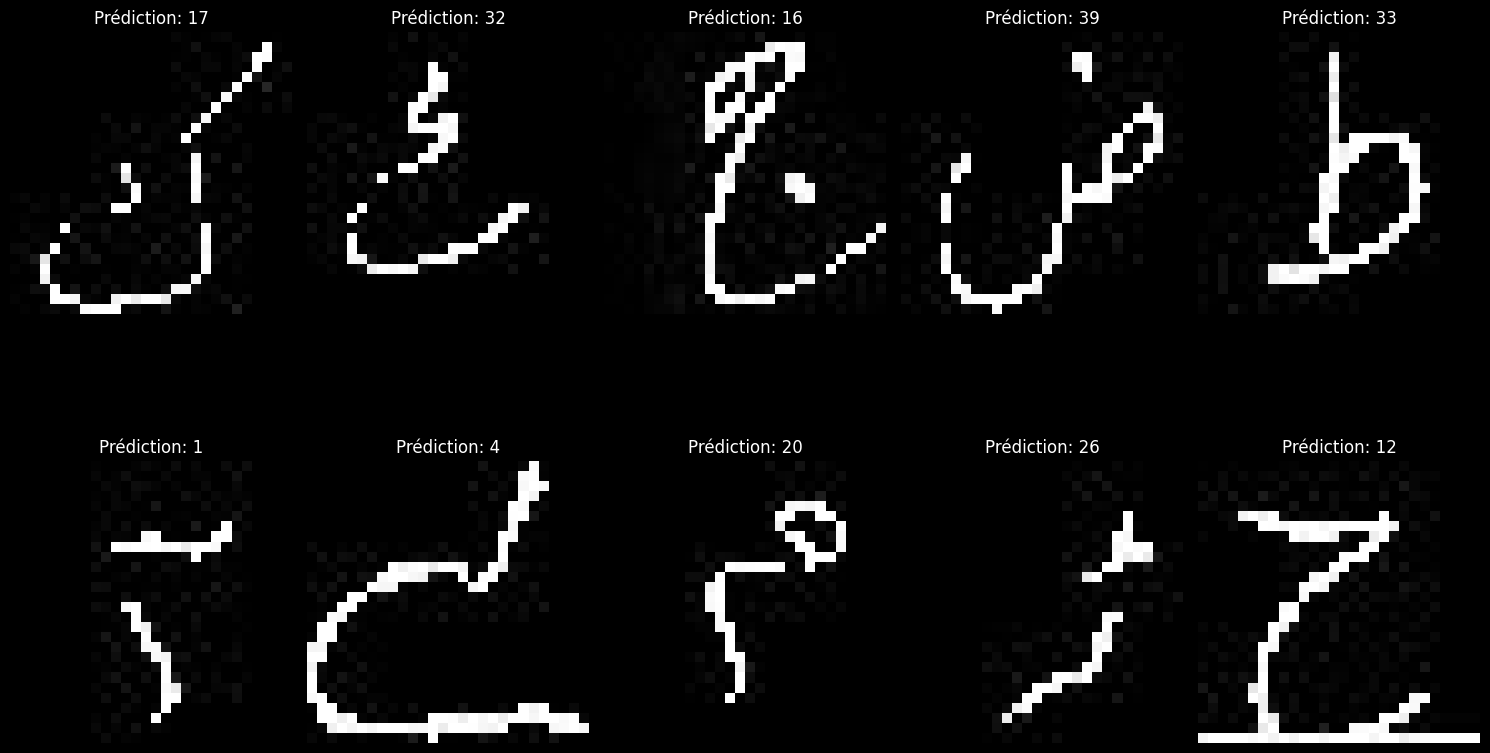
\includegraphics[width=0.7\textwidth]{figures/Prédiction.png}
\caption{Exemple de caractères ourdous prédicte}
\label{fig:urdu_chars_prédicte}
\end{figure}